\documentclass[a4paper,12pt]{article}
\usepackage[utf8]{inputenc}
\usepackage{graphicx}
\usepackage{hyperref}
\usepackage{geometry}
\usepackage{longtable}
\usepackage{amsmath}
\usepackage{listings}
\usepackage{xcolor}
\usepackage{fancyhdr}
\usepackage{titlesec}

% Configuración de márgenes
\geometry{top=2.5cm, bottom=2.5cm, left=2.5cm, right=2.5cm}

% Configuración de encabezado y pie de página
\pagestyle{fancy}
\fancyhead{}
\fancyfoot{}
\fancyhead[L]{Sistema de Generación Automática de Exámenes}
\fancyfoot[C]{\thepage}

% Configuración de títulos
\titleformat{\section}{\large\bfseries}{\thesection}{1em}{}
\titleformat{\subsection}{\normalsize\bfseries}{\thesubsection}{1em}{}
\titleformat{\subsubsection}{\normalsize\itshape}{\thesubsubsection}{1em}{}

% Configuración de código fuente
\lstset{
  basicstyle=\ttfamily\footnotesize,
  breaklines=true,
  commentstyle=\color{gray},
  keywordstyle=\color{blue},
  stringstyle=\color{red},
  numbers=left,
  numberstyle=\tiny\color{gray}
}

\begin{document}

\begin{titlepage}
    \centering
    \vspace{1in}
    {\Huge \bfseries Sistema de Generación Automática de Exámenes \par}
    \vspace{1.5in}
    {\Large John García Muñoz - Grupo: 311 CI :03012369124  \par}
    {\Large Victor Hugo Pacheco Fonseca - Grupo: 311 CI :03021580729 \par}
    {\Large Jose Agustín del Toro González - Grupo: 312 CI :01062069124 \par}
    \vfill
    {\Large \today \par}
\end{titlepage}

\tableofcontents
\newpage

\section{Introducción}

\subsection{Objectivo del Proyecto}
El sistema de Gestión para la Generación Automática de Exámenes está diseñado para proporcionar una solución integral en la administración y evaluación de exámenes en instituciones educativas. Este sistema tiene como objetivo principal optimizar el proceso de creación de exámenes, simplificar la gestión de preguntas y proporcionar herramientas avanzadas de análisis y reportes de desempeño estudiantil. Al integrar estas funcionalidades, el sistema busca reducir significativamente la carga administrativa de los profesores y mejorar la precisión y la calidad en la evaluación de los estudiantes.


\newpage
\section{Requerimientos}
A continuación los requerimientos técnicos y de software necesarios para la ejecución del proyecto.

\subsection{Requerimientos Técnicos}
\subsubsection{Hardware}
\begin{itemize}
	\item Procesador con al menos 2 GHz de velocidad..
	\item Memoria RAM mínima de 4 GB, suficiente para entornos de desarrollo
	locales.
	\item Espacio en disco de al menos 2 GB para almacenamiento del código,
	dependencias.
\end{itemize}

\subsubsection{Sistema Operativo}
\begin{itemize}
    \item Windows.
    \item Linux.
    \item macOs.
\end{itemize}

\subsection{Requerimientos de Software.}
Backend.
\begin{itemize}
	\item Python : Versión 3.8 o superior.
	\item Django: Versión 3.2 o superior.
	\item SQLite como base de datos.
	\item El archivo requirements.txt contenido en la carpeta backend contiene el resto de todos los paquetes y librerías que se necesita para ejecutar el proyecto,para instalarlos de forma automática ejecutar el comando: pip install -r requirements.txt.
\end{itemize}
FrontEnd.
\begin{itemize}
	\item Node.js 16 o superior.
\end{itemize}

\section{Instalación}

\section{Descripción General del Producto}

El Sistema de Gestión de Exámenes Automáticos es una herramienta versátil que se adapta a las necesidades de diferentes actores dentro de una institución educativa. Sus principales funciones incluyen:
\begin{itemize}
	
	\item \textbf{Gestión de Preguntas}: Facilita la creación y clasificación de preguntas, asegurando que estén organizadas de manera eficiente y fácilmente accesibles para su uso en exámenes.(Ver Figure 1)
	\item \textbf{Generación Automática de Exámenes}: Permite a los profesores crear exámenes de manera automática seleccionando preguntas de una base de datos organizada por temas y niveles de dificultad.(Ver Figure 2)
	\item \textbf{Validación de Exámenes}: Permite al jefe de asignatura (un profesor cualificado) validar los exámenes antes de su publicación, asegurando la calidad y coherencia del contenido.(Ver Figure 3)
		\item \textbf{Calificación de exámenes}: Los profesores pueden calificar y los exámenes hechos por sus estudaintes.(Ver Figure 4)
	\item \textbf{Informes y Estadísticas}: Ofrece informes sobre la utilización de preguntas, el desempeño de los estudiantes y la distribución de preguntas por tema y dificultad, lo que facilita la toma de decisiones informadas.
\end{itemize}


\begin{figure}[h]  % El entorno figure facilita la colocación y manejo de las imágenes
	\centering     % Centra la imagen
	
\includegraphics[width=0.5\textwidth]{agregarPregunta.png}
	\caption{Agregar pregunta.}
	\label{fig:mi_imagen}
\end{figure}

\begin{figure}[h]  % El entorno figure facilita la colocación y manejo de las imágenes
	\centering     % Centra la imagen
	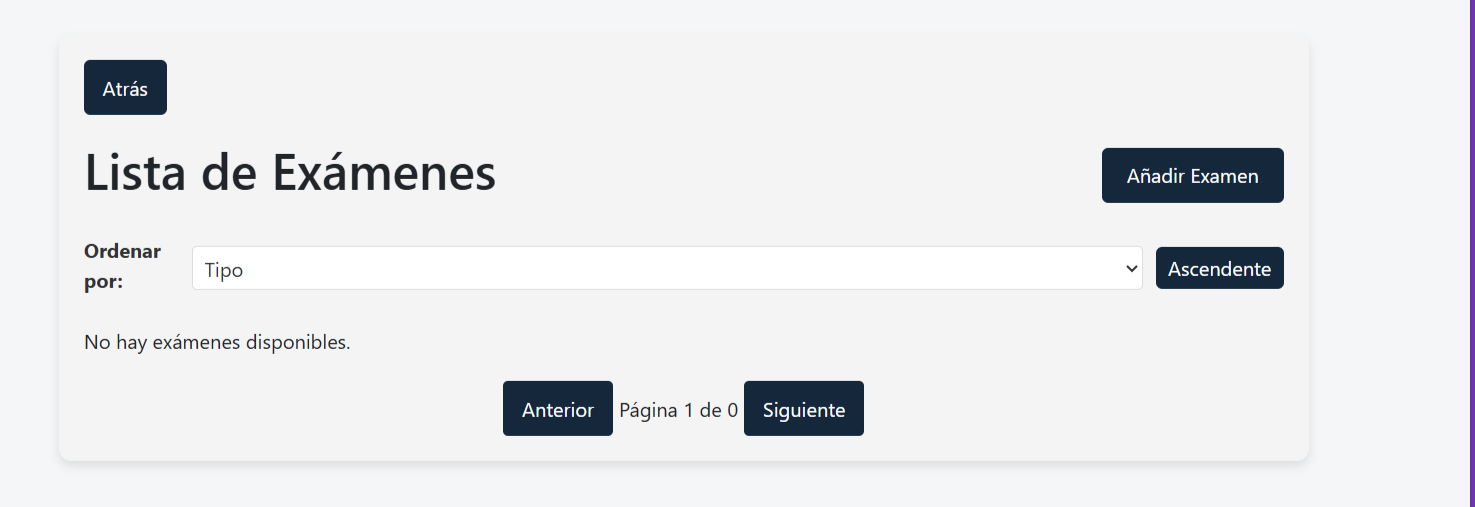
\includegraphics[width=0.5\textwidth]{agregarExamen.png}
	\caption{Agregar exámen.}
	\label{fig:mi_imagen}
\end{figure}

\begin{figure}[h]  % El entorno figure facilita la colocación y manejo de las imágenes
	\centering     % Centra la imagen
	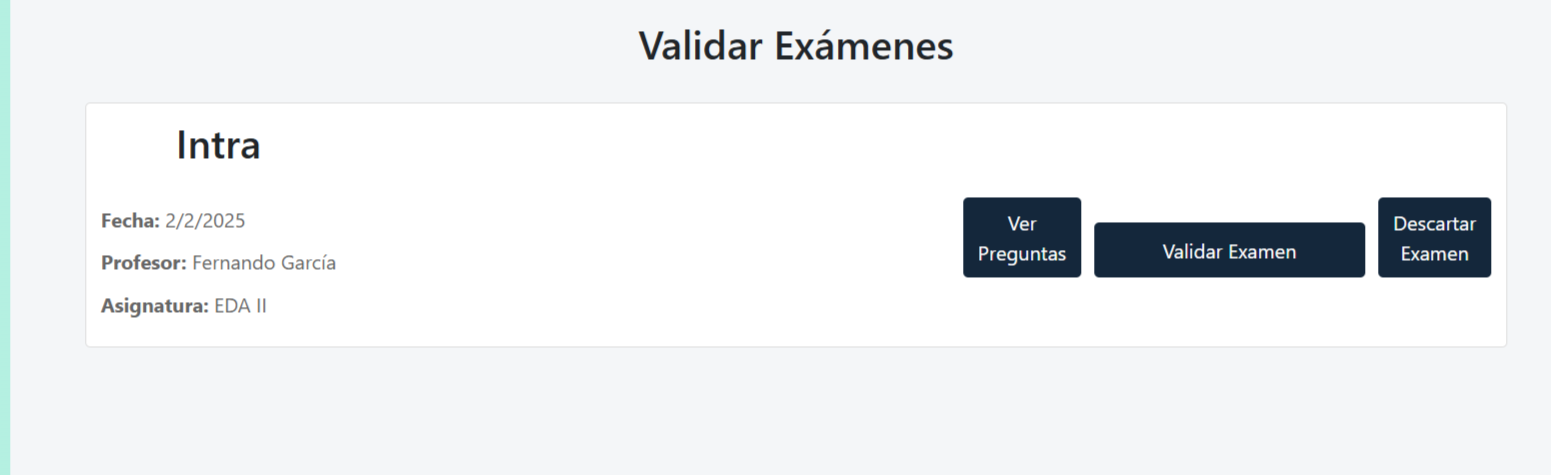
\includegraphics[width=0.5\textwidth]{ValidarExamen.png}
	\caption{Validar exámen.}
	\label{fig:mi_imagen}
\end{figure}

\begin{figure}[h]  % El entorno figure facilita la colocación y manejo de las imágenes
	\centering     % Centra la imagen
	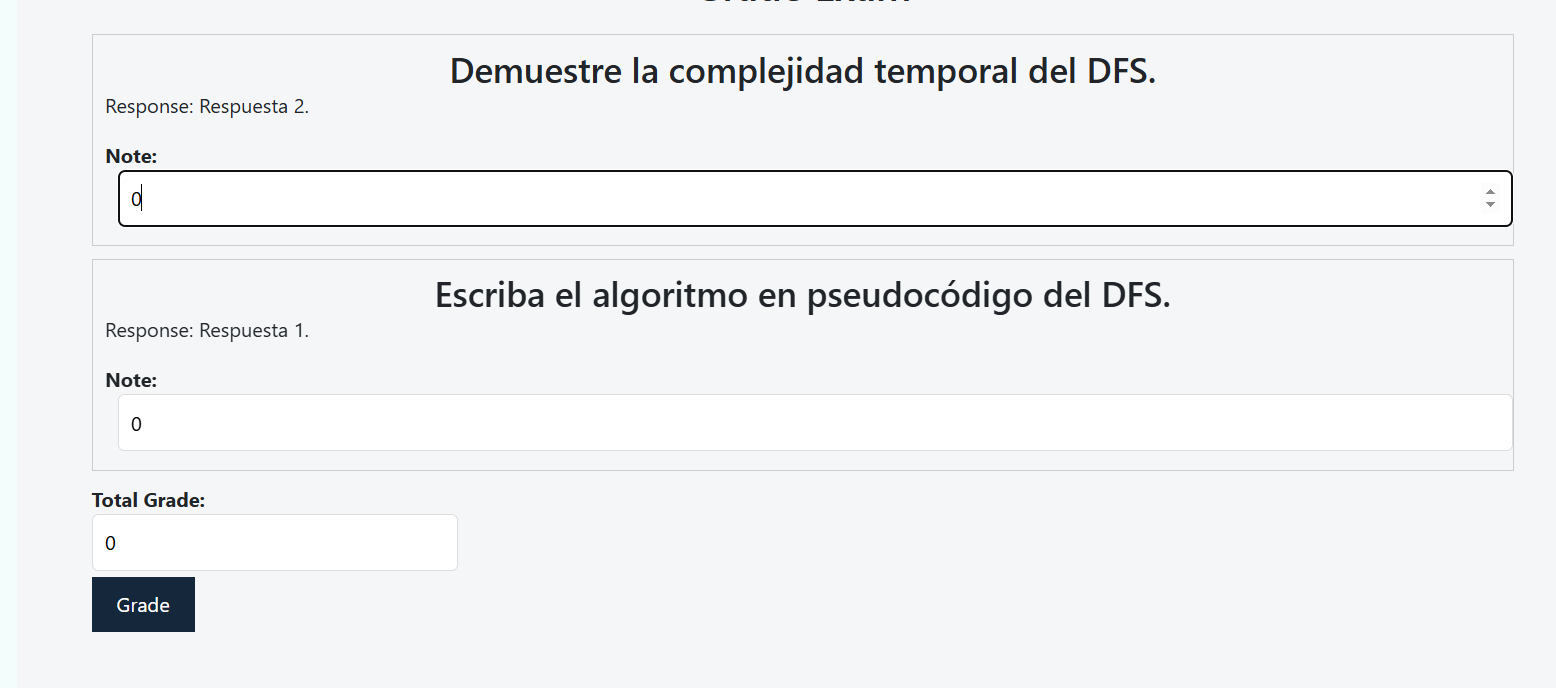
\includegraphics[width=0.5\textwidth]{CalificarExamen.png}
	\caption{Calificar exámen.}
	\label{fig:mi_imagen}
\end{figure}


\newpage
\subsection{Descripción de los Actores}
\begin{itemize}
    \item \textbf{Profesor}: Actor principal que crea, valida y califica exámenes y gestiona preguntas. Los profesores tienen acceso a todas las herramientas necesarias para gestionar exámenes y evaluar a los estudiantes de manera eficiente.
    \item \textbf{Estudiante}: Toma los exámenes y recibe una calificación de su profesor.Ademas puede solicitar la recalificación de un exámen y especificar que profesor la va a ser. Los estudiantes pueden acceder a sus resultados y consultar sus estadísticas.
	\item \textbf{Administrador}: Gestiona las asignaturas,temas y cursos existentes, así como a los usuarios, su función es controlar los parámetros administrativos más generales que no deben quedar en manos de los usuarios.
\end{itemize}





\end{document}


